\begin{figure}[b]
    % \centering
    \begin{minipage}[b]{0.48\textwidth}
   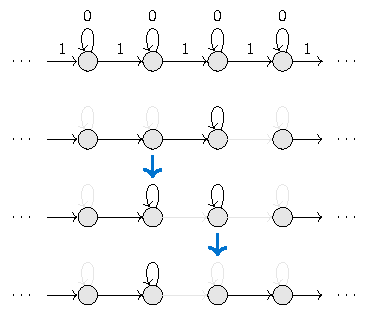
\includegraphics{figures/loop.pdf}
    %     \pgfmathsetmacro{\xdist}{1.1}
    % \pgfmathsetmacro{\ydist}{-1.2*\xdist}
        % \begin{tikzpicture}[
        %     scale=1, auto, node distance=1cm, 
        %     every edge/.style={draw, <-, looseness=20},
        %     state/.style={circle, fill=mylightgrey, draw=black, text=black},
        %     changebox/.style={draw=blue!70!black, very thick, rounded corners, inner sep=2pt}
        % ]
        
        % % -------------------------------------------------
        % % Row 0 : initial policy (all states choose move)
        % % -------------------------------------------------
        % % \node at (-2.2,  0.0) {$\pi^{(0)}$};
        % \node[font=\footnotesize] (l0) at (-\xdist, 0.0) {$\cdots$};
        
        % \node[state] (a1) at (0.0, 0.0) {};
        % \node[state] (a2) at (\xdist, 0.0) {};
        % \node[state] (a3) at (2*\xdist, 0.0) {};
        % \node[state] (a4) at (3*\xdist, 0.0) {};
        
        % \node[font=\footnotesize] (r0) at (4*\xdist, 0.0) {$\cdots$};
        
        % % move actions (active)
        % \draw[->] ($(l0.east)+(0.10,0)$) -- node[midway, above, font=\footnotesize] {$1$} (a1.west);
        % \draw[->] (a1.east) -- node[midway, above, font=\footnotesize] {$1$} (a2.west);
        % \draw[->] (a2.east) -- node[midway, above, font=\footnotesize] {$1$} (a3.west);
        % \draw[->] (a3.east) -- node[midway, above, font=\footnotesize] {$1$} (a4.west);
        % \draw[->] (a4.east) -- node[midway, above, font=\footnotesize] {$1$} ($(r0.west)+(-0.10,0)$);
        
        % % stay actions (inactive)
        % \path[->]
        %     (a1) edge[out=110, in=70, loop, looseness=12, draw=black]
        %         node[pos=0.5, above, text=black, font=\footnotesize] {$0$} (a1)
        %     (a2) edge[out=110, in=70, loop, looseness=12, draw=black]
        %         node[pos=0.5, above, text=black, font=\footnotesize] {$0$} (a2)
        %     (a3) edge[out=110, in=70, loop, looseness=12, draw=black]
        %         node[pos=0.5, above, text=black, font=\footnotesize] {$0$} (a3)
        %     (a4) edge[out=110, in=70, loop, looseness=12, draw=black]
        %         node[pos=0.5, above, text=black, font=\footnotesize] {$0$} (a4);
        
        % % \draw[->, dotted, thick]
        % %     ($(r0.south)+(0,-0.45)$)
        % %     to[out=0, in=-180, looseness=1]
        % %     ($(l0.south)+(0,-0.45)$);
        % % -------------------------------------------------
        % % Row 1 : state s_{i+1} switches to stay
        % % -------------------------------------------------
        % % \node at (-2.2, -1.9) {$\pi^{(1)}$};
        % \node[font=\footnotesize] (l1) at (-\xdist, \ydist) {$\cdots$};
        
        % \node[state] (b1) at (0.0, \ydist) {};
        % \node[state] (b2) at (\xdist, \ydist) {};
        % \node[state] (b3) at (2*\xdist, \ydist) {};
        % \node[state] (b4) at (3*\xdist, \ydist) {};
        
        % \node[font=\footnotesize] (r1) at (4*\xdist, \ydist) {$\cdots$};
        
        % % move actions
        % \draw[->] ($(l1.east)+(0.10,0)$) -- (b1.west);
        % \draw[->] (b1.east) -- (b2.west);
        % \draw[->] (b2.east) -- (b3.west);
        % \draw[->, draw=mylightgrey] (b3.east) -- (b4.west);
        % \draw[->] (b4.east) -- ($(r1.west)+(-0.10,0)$);
        
        % % stay actions
        % \path[->]
        %     (b1) edge[out=110, in=70, loop, looseness=12, draw=mylightgrey] (b1)
        %     (b2) edge[out=110, in=70, loop, looseness=12, draw=mylightgrey] (b2)
        %     (b3) edge[out=110, in=70, loop, looseness=12, draw=black] (b3)
        %     (b4) edge[out=110, in=70, loop, looseness=12, draw=mylightgrey] (b4);
        
        % % \node[changebox, fit=(b2)] (box1) {};
        
        % % -------------------------------------------------
        % % Row 2 : state s_{i+2} also switches to stay
        % % -------------------------------------------------
        % % \node at (-2.2, -1.9) {$\pi^{(1)}$};
        % \node[font=\footnotesize] (l2) at (-\xdist, 2*\ydist) {$\cdots$};
        
        % \node[state] (c1) at (0.0, 2*\ydist) {};
        % \node[state] (c2) at (\xdist, 2*\ydist) {};
        % \node[state] (c3) at (2*\xdist, 2*\ydist) {};
        % \node[state] (c4) at (3*\xdist, 2*\ydist) {};
        
        % \node[font=\footnotesize] (r2) at (4*\xdist, 2*\ydist) {$\cdots$};
        
        % % move actions
        % \draw[->] ($(l2.east)+(0.10,0)$) -- (c1.west);
        % \draw[->] (c1.east) -- (c2.west);
        % \draw[->, draw=mylightgrey] (c2.east) -- (c3.west);
        % \draw[->, draw=mylightgrey] (c3.east) -- (c4.west);
        % \draw[->] (c4.east) -- ($(r2.west)+(-0.10,0)$);
        
        % % stay actions
        % \path[->]
        %     (c1) edge[out=110, in=70, loop, looseness=12, draw=mylightgrey] (c1)
        %     (c2) edge[out=110, in=70, loop, looseness=12, draw=black] (c2)
        %     (c3) edge[out=110, in=70, loop, looseness=12, draw=black] (c3)
        %     (c4) edge[out=110, in=70, loop, looseness=12, draw=mylightgrey] (c4);
        
        % % \node[changebox, fit=(b2) (c2)] (box2) {};
        
        % % -------------------------------------------------
        % % Row 3 : state s_{i+3} also switches to stay
        % % -------------------------------------------------
        % % \node at (-2.2, -5.7) {$\pi^{(3)}$};
        % \node[font=\footnotesize] (l3) at (-\xdist, 3*\ydist) {$\cdots$};
        
        % \node[state] (d1) at (0.0, 3*\ydist) {};
        % \node[state] (d2) at (\xdist, 3*\ydist) {};
        % \node[state] (d3) at (2*\xdist, 3*\ydist) {};
        % \node[state] (d4) at (3*\xdist, 3*\ydist) {};
        
        % \node[font=\footnotesize] (r3) at (4*\xdist, 3*\ydist) {$\cdots$};
        
        % % move actions
        % \draw[->] ($(l3.east)+(0.10,0)$) -- (d1.west);
        % \draw[->] (d1.east) -- (d2.west);
        % \draw[->, draw=mylightgrey] (d2.east) -- (d3.west);
        % \draw[->] (d3.east) -- (d4.west);
        % \draw[->] (d4.east) -- ($(r3.west)+(-0.10,0)$);
        
        % % stay actions
        % \path[->]
        %     (d1) edge[out=110, in=70, loop, looseness=12, draw=mylightgrey] (d1)
        %     (d2) edge[out=110, in=70, loop, looseness=12] (d2)
        %     (d3) edge[out=110, in=70, loop, looseness=12, draw=mylightgrey] (d3)
        %     (d4) edge[out=110, in=70, loop, looseness=12, draw=mylightgrey] (d4);
        
        % % \node[changebox, fit=(c3) (d3)] (box3) {};
        
        % % -------------------------------------------------
        % % Blue arrows showing where the policy changes next
        % % -------------------------------------------------
        % % \draw[->, blue!70!black, very thick] (box1.south) -- (box2.north);
        % % \draw[->, blue!70!black, very thick] (box2.south) -- (box3.north);

        % \draw[->, very thick, CambridgeCoreBlue]
        %     ($(b2.south)+(0,-0.1)$) -- ($(c2.north)+(0,0.5)$);
        
        % \draw[->, very thick, CambridgeCoreBlue]
        %     ($(c3.south)+(0,-0.1)$) -- ($(d3.north)+(0,0.5)$);
        % \end{tikzpicture}
    \vspace{0.5cm}
    \caption{The MDP forms a connected chain of 13 states, each with two actions. 
    As in \autoref{fig: explain loop on-policy bias MDP}, solutions cycle between suboptimal policies that only contain 1 or 2 suboptimal actions.
    The suboptimal action propagates backwards relative to the state-transitions.}
    \label{fig: long MDP}
    \end{minipage}
    \hfill
    \begin{minipage}[b]{0.48\textwidth}
   % \begin{tikzpicture}
   %  \begin{axis}[
   %      width=\linewidth,
   %      height=5.4cm,
   %      % axis equal image,
   %      xmin=-0.007, xmax=0.0120,
   %      ymin=-0.02, ymax=0.0080,
   %      grid=none,
   %      grid style={line width=0.2pt, draw=gray!35},
   %      % major grid style={line width=0.3pt, draw=gray!45},
   %      tick label style={font=\small},
   %      title={Deterministic solution in $s_1$},
   %      xlabel={$q_k(s_1,a_*)-\widehat q$},
   %      ylabel={$q_k(s_1,\bar a)-\widehat q$},
   %      % legend style={draw=none, fill=none, font=\small, at={(0.65,.3)}, anchor=north},
   %      % legend columns=1,
   %      scaled ticks=true,
   %      every x tick scale label/.style={
   %          at={(axis description cs:1.0,0.0)},
   %          anchor=north,
   %          font=\small
   %      },
   %      every y tick scale label/.style={
   %          at={(axis description cs:0,1.0)},
   %          anchor=south,
   %          font=\small
   %      },
   %      % legend cell align={left}
   %      ]
   %      \addplot[forget plot, CambridgeCoreBlue]
   %          table[col sep=comma, x=x, y=y]{figures/deterministic_phase_path_s1.csv};
   %      % \addlegendentry{trajectory from CSV}
   %      \addplot[forget plot, only marks, mark=*, mark size=2.2pt, black]
   %          table[col sep=comma, x=x, y=y]{figures/spiral_initial_s1.csv}
   %          node[pos=0, right] {$q_0$};
   %      % \addlegendentry{initial}
   %      % \addplot+[forget plot, only marks, mark=x, mark size=3.0pt, line width=0.8pt]
   %      %     coordinates {(0,0)};
   %      % \addlegendentry{$(\widehat q,\widehat q)$}
   %      \addplot[forget plot, only marks, mark=square*, mark size=2.1pt]
   %          table[col sep=comma, x=x, y=y]{figures/spiral_final_s1.csv};
   %      % \addlegendentry{after 1000 cycles}
   %      \addplot[forget plot, dotted, black, domain=-0.010:0.02, samples=2] {x};
   %      % \addlegendentry{zero-gap line}
   %  \end{axis}
   %  \end{tikzpicture} 
   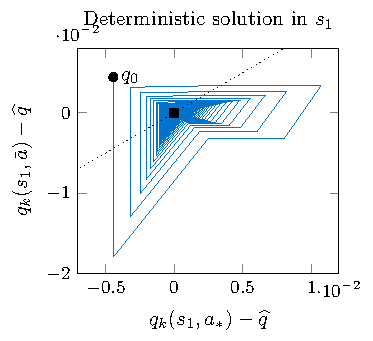
\includegraphics{figures/spiral-fig.pdf}
    \caption{Mean-field solutions of FV/SA MCES robustly converge to a suboptimal point $(\widehat q, \widehat q)$ derived in Appendix~\ref{sec:balance-general}.
    % Solutions
    % Deterministic expected-update spiral for state $s_1$. 
    Solution is initialised with counts $n_0(s,a_*):=10$ and $n_0(s,\bar a) := 5$.
    The dotted line corresponds to the boundary where $q(s_1,a_*)=q(s_1,\bar a)$}
    \label{fig:spiral}
    \end{minipage}
\end{figure}